% Mirror: https://github.com/SIGma-UIUC/presentation-format
% --------------------------------------------------------------------
% This is a simple Beamer document that uses beamerthemesigma.sty
% Reading the comments should help you create a presentation even if
% you've never used Beamer before.
% --------------------------------------------------------------------

% Set our document class to Beamer
\documentclass[aspectratio=169]{beamer}
%\documentclass[aspectratio=169, handout]{beamer}
% Add handout option to ignore pauses

% From Jeff E
\usepackage{algo}
% Some more macros
\usepackage{sigmastyle}
\usepackage{amssymb}
\usepackage{subcaption}
\usepackage{wrapfig}
\usepackage{tcolorbox}

\usepackage{forest}
\forestset{
  default preamble={
    for tree={
        grow=south,
        circle, draw, minimum size=3ex, inner sep=1pt,
        s sep=3mm,
    }
  }
}
\usepackage{adjustbox}

% Quotes are fun, find some to use!
\font\eightss=cmssq8
\font\eightssi=cmssqi8
\newcommand\quoteAuthor[2]{\begingroup
  \baselineskip 10pt
  \parfillskip 0pt
  \interlinepenalty 10000 % not needed in example
  \leftskip 0pt plus 40pc minus \parindent
  \let\rm=\eightss
  \let\sl=\eightssi
  \everypar{\sl}#1\par
  \nobreak\smallskip
  \noindent\rm--- #2\unskip\par
  \endgroup}
\newcommand\quoteAuthorDate[3]{\begingroup
  \baselineskip 10pt
  \parfillskip 0pt
  \interlinepenalty 10000 % not needed in example
  \leftskip 0pt plus 40pc minus \parindent
  \let\rm=\eightss
  \let\sl=\eightssi
  \everypar{\sl}#1\par
  \nobreak\smallskip
  \noindent\rm--- #2\unskip\enspace(#3)\par
  \endgroup}

\newcommand{\TT}{\mathcal{T}}

% Set a title
\title{(Pseudo)Random Number Generation}

% Set a subtitle if you desire
% \subtitle{[TAOCP 5 8.9.10.11]}

% Whoever worked on the presentation:
\author{Krish}

% Date looks ugly, so leave blank
\date{}

% An institute name, if you're so inclined
% \institute{University of Illinois Urbana-Champaign}

% Use the SIGma theme for this Beamer presentation
\usetheme{sigma}
% --------------------------------------------------------------------

% Begin document
\begin{document}

% Beamer calls each slide a "frame", defined within the environment:
% \begin{frame}
%   <frame content here>
% \end{frame}

% This frame is just the title.
\begin{frame}
\titlepage
\end{frame}

% A frame with the table of contents.
% This frame's title is "Outline".
\begin{frame}{Outline}
  \tableofcontents
\end{frame}

% \begin{frame}{Updates!}
%   % Let's put some real content in this frame:
%   Weekly updates:
%   \begin{itemize}
%     \item SIGma is an excellent SIG.
%     \item I'm out of ideas for updates.
%   \end{itemize}
% \end{frame}

% Start a section: *sections* (subsections, etc.) are what show up in the TOC.
\section{Introduction}
% Section pages can be printed thus:
% \frame{\sectionpage}
% There's a way to automate this, see:
% https://tex.stackexchange.com/questions/178800/creating-sections-each-with-title-pages-in-beamers-slides/178803

\begin{frame}{Introduction}
  
  \begin{tcolorbox}[title=Problem,colbacktitle=sigma@mainblue]
    
  How can computers, which are purely deterministic, generate random numbers?
  \end{tcolorbox}

  Before discussing this, let's talk about randomness in nature. \pause
  
  Nature is full of random fluctuations: rate of radioactive decay, the number of faces on a pebble, thermal noise, etc. \pause

  It is possible, in theory, to measure one such random event and use that to generate a random number.
  \begin{itemize}
    \item This does pose some issues when it comes to generating massive numbers, as well as being very inefficient and slow.
  \end{itemize} \pause

  Thus, we must turn to algorithms to generate \textit{pseudorandom} numbers.

\end{frame}

\begin{frame}{What Does "Pseudorandom" Even Mean?}
  A pseudorandom number is defined as a number that "appears to be statistically random, despite having been produced by a completely deterministic and repeatable process" (Wikipedia). \pause

  Basically, at first glance, a pseudorandom number appears random, but after enough numbers have been generated, a clear pattern emerges. \pause

  We can visualize this using random walks, which show the progression and relation between a set of generated numbers by plotting the distance between two consecutive numbers in a set of numbers.
\end{frame}

\begin{frame}{Truly Random Visualization}
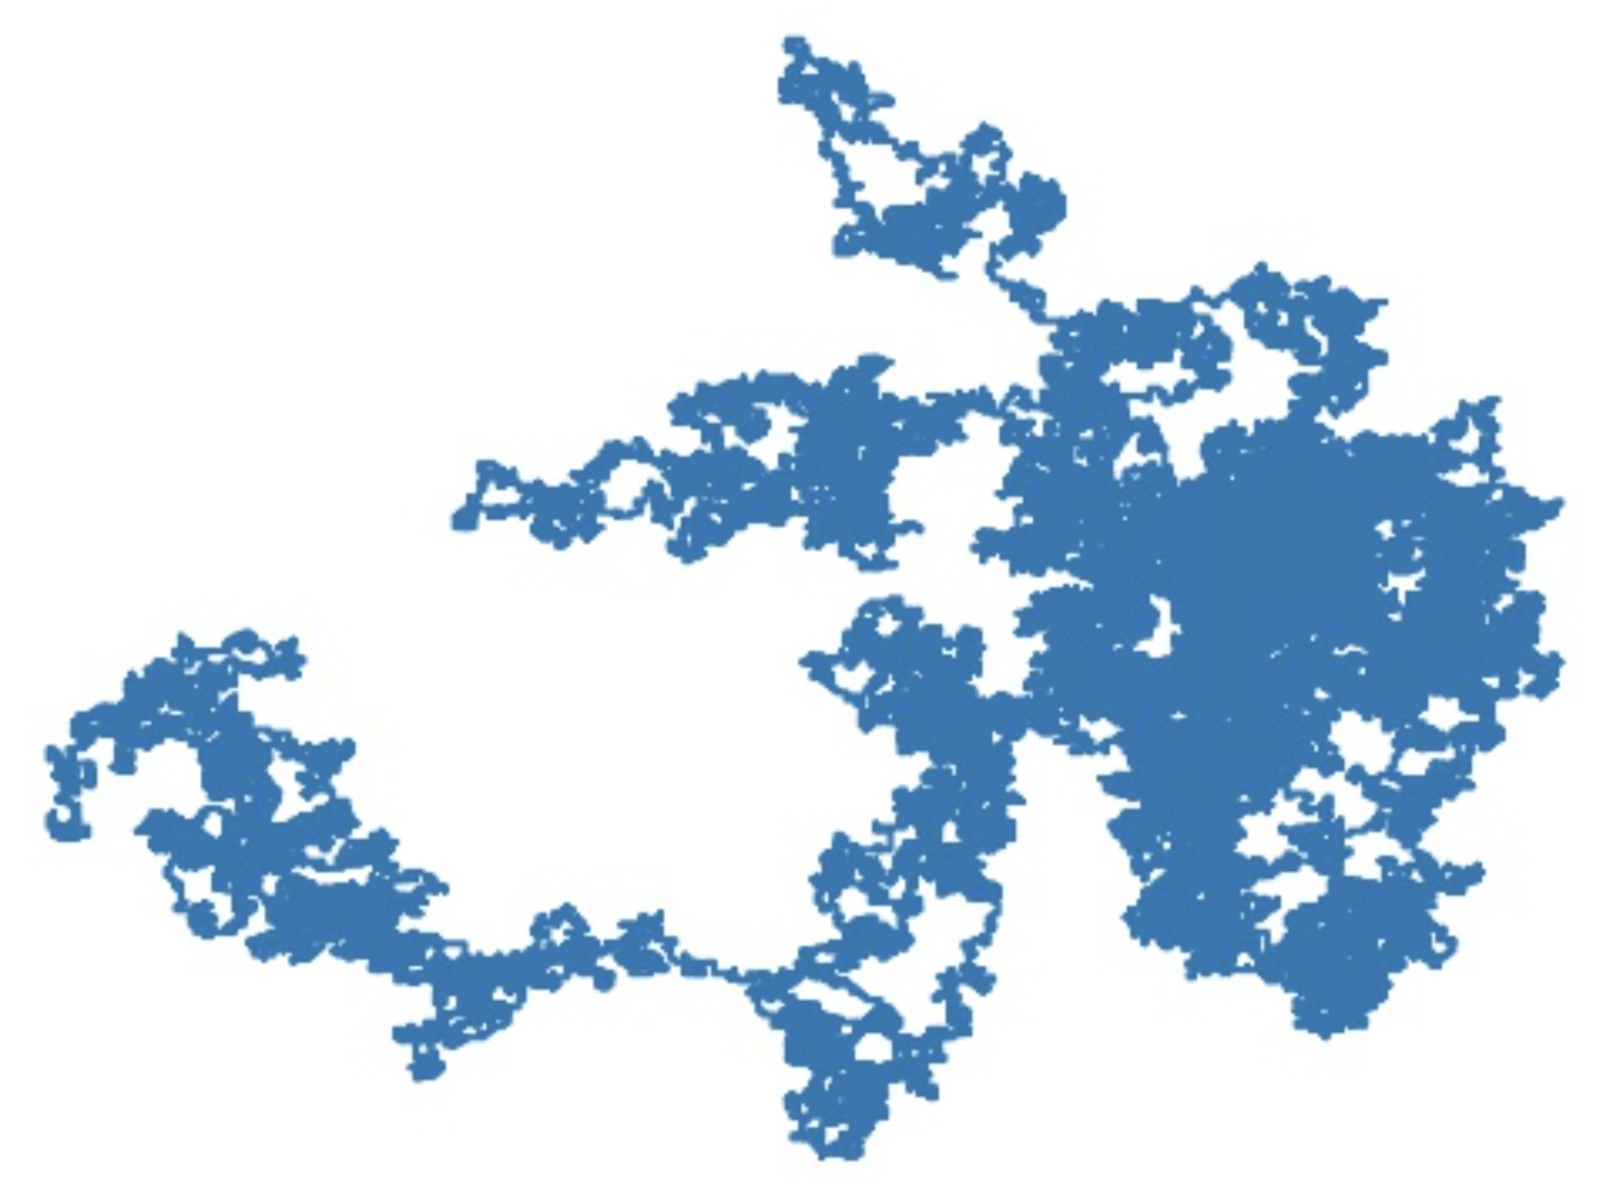
\includegraphics[width=0.8\textwidth]{random.png}
\end{frame}

\begin{frame}{Pseudorandom Visualization}
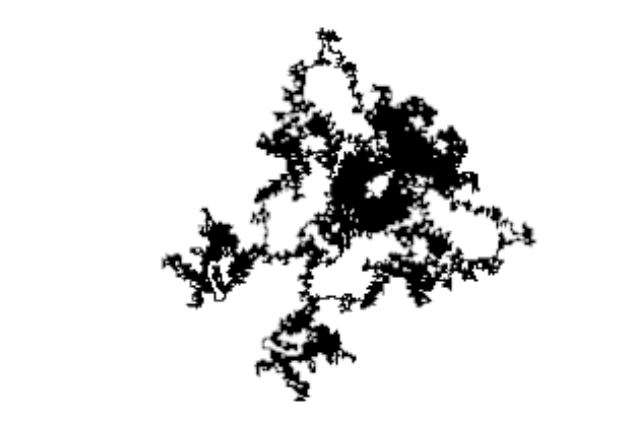
\includegraphics[width=0.8\textwidth]{pseudorandom.png}
\end{frame}

\section{Middle Squares Method}
\begin{frame}{Middle Squares Method}
\begin{enumerate}
    \item Start by choosing a seed. The last three digits of the Unix time as I'm making this are 186, so that's our seed number. \pause
    \item Now square this number and select as many middle digits as needed (here we're doing 3). $186^2 = 34596$, so our next seed is 459. \pause 
    \item Repeat using this number as the new seed. \pause
\end{enumerate}
Thus, to generate random 3-digit numbers with a seed of 186, we get:
$186^2 = 34596 \rightarrow 459$, $459^2 = 210681 \rightarrow 068$, $68^2 = 4624 \rightarrow 624$, $624^2 = 389376 \rightarrow 937$, $937^2 = 877969 \rightarrow 796$, and so on. \pause

Once you get a repeat number, it's easy to see that the numbers will start to repeat from there. Some seeds will have a longer period than others.


\end{frame}
\section{Linear Congruential Generator}
\begin{frame}{Linear Congruential Generator (LCG)}
The LCG is another simple pseudorandom number generator.

The general LCG formula is:
\[X_{n+1} = (a X_n + c)\mod m\] \pause
Where:
\begin{itemize}
    \item \(X_n\) is the current seed
    \item \(X_{n+1}\) is the next pseudorandom number
    \item \(a\) is the multiplier
    \item \(c\) is the increment
    \item \(m\) is the modulus
    \item Assume all are non-zero
\end{itemize}
\end{frame}

\begin{frame}{Example LCG Computation}
Given arbitrary parameters: $m = 79, \quad a = 43, \quad c = 15, \quad X_0 = 21$
\begin{enumerate}
    \item $X_1 = (43 \cdot 21 + 15) \mod 79$
    
        $43 \cdot 21 = 903  \rightarrow  903 + 15 = 918  \rightarrow  918 \mod 79 = 63$
        
        $X_1 = 63$
    \item $X_2 = (43 \cdot 63 + 15) \mod 79$
        $43 \cdot 63 = 2709  \rightarrow  2709 + 15 = 2724  \rightarrow  2724 \mod 79 = 9$
        
        $X_2 = 9$
    \item $X_3 = (43 \cdot 9 + 15) \mod 79$
    
        $43 \cdot 9 = 387  \rightarrow  387 + 15 = 402  \rightarrow  402 \mod 79 = 7$
        
        $X_3 = 7$
\end{enumerate}
We get a sequence of 21, 63, 9, 7, 0, 15, 34, and so on.

\end{frame}

\section{XorShift}

\begin{frame}{XorShift}
General Process:

\begin{enumerate}
    \item Pick a seed and convert it to binary.
    \item Perform a bit shift either left or right and any amount.
    \item Perform the Xor operation ($\oplus$) on the numbers in steps $1$ and $2$.
    \item Repeat steps $1$ -- $3$ as many times as you want, reversing the direction of the bit shift each time.
    \item Convert the final number back to decimal.
\end{enumerate}
\end{frame}

\begin{frame}{Example with Arbitrary Seed 3146505}
\begin{table}[h]

\begin{tabular}{|l|l|}
\hline
\textbf{Step} & \textbf{Result of Operation} \\
\hline
Initial & 
\textcolor{blue}{0000 0000 0011 0000 0000 0011 0000 1001} \\
\hline
Left Shift $\ll 13$ & 
\textcolor{red}{0001 1000 0000 0000 0000 0000 0000 0000} \\
\hline
Xor1: $12345 \oplus (12345 \ll 13)$ & 
\textcolor{green}{0001 1000 0011 0000 0000 0011 0000 1001} \\
\hline
Right Shift $\gg 17$ & 
\textcolor{purple}{0000 0000 0000 0001 1000 0000 0000 0000} \\
\hline
Xor2: $\text{Previous} \oplus (\text{Previous} \gg 17)$ & 
\textcolor{orange}{0001 1000 0011 0001 1000 0011 0000 1001} \\
\hline
Left Shift $\ll 5$ & 
\textcolor{brown}{0011 0000 0110 0010 0000 0110 0010 0000} \\
\hline
Xor3: $\text{Previous} \oplus (\text{Previous} \ll 5)$ & 
\textcolor{teal}{0010 1000 0101 0011 1000 0101 0010 1001} \\
\hline

\end{tabular}
\end{table}
\end{frame}

\begin{frame}{Results}
  
\begin{table}[h]

\begin{tabular}{|c|c|c|c|}
\hline
Iteration & Initial Seed & Operations & Result \\
\hline
0 & 3146505 & Initial seed & 3146505 \\
1 & 3146505 & $3146505 \oplus (3146505 \ll 13)$ & 405799689 \\
2 & 405799689 & $405799689 \oplus (405799689 \gg 17)$ & 405897993 \\
3 & 405897993 & $405897993 \oplus (405897993 \ll 5)$ & 676562217 \\
\hline
\end{tabular}
\end{table}


Pseudorandom number: 676562217
\end{frame}

\begin{frame}{Summary}
Middle Squares, LCG, and XorShift are three fairly simple pseudorandom number generation algorithms. \pause

All three can be completed in constant time, making them suitable for real-time simulation number generation. \pause

This does mean that neither is great for cryptographic purposes, which often use many complex processes like entropy pools, block ciphers, and sometimes even truly random numbers from physical processes as I mentioned earlier. I highly recommend reading up on these as they are very interesting!
\end{frame}

% Asking questions is fun but we should answer some first
\begin{frame}{}
      \begin{center}
    {\color{sigma@mainblue} \LARGE Questions?}
  \end{center}
\end{frame}

\end{document}